\begin{figure}
\caption{Cost-Push Shock Impulse Responses}\label{fg:irf_cost}
\vspace*{1pc}
\begin{tabular}{cc}
\multicolumn{2}{c}{Case 2: Learning with RE Initial Conditions}\\ \\
Output Gap & Inflation \\ 
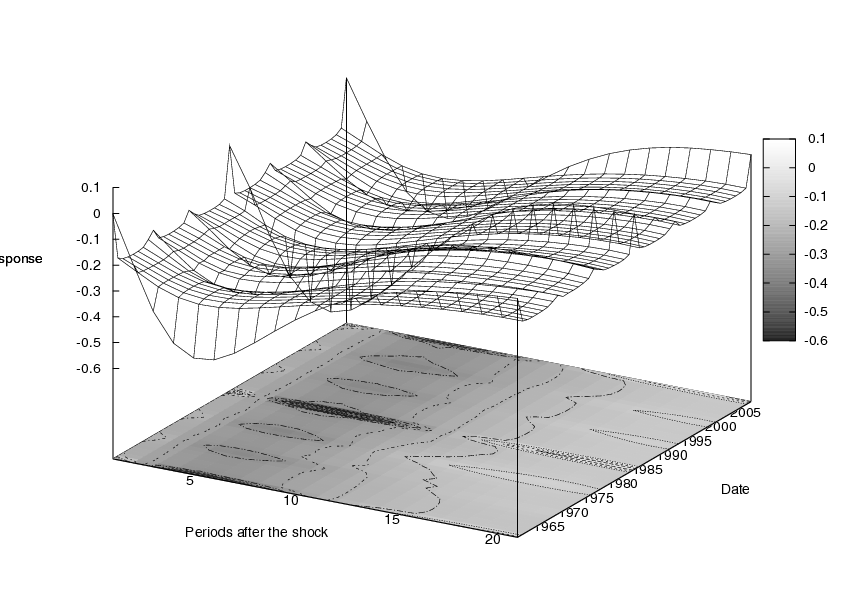
\includegraphics[scale=0.25]{results_reallinit/Output_costshock_irf3d.png} & 
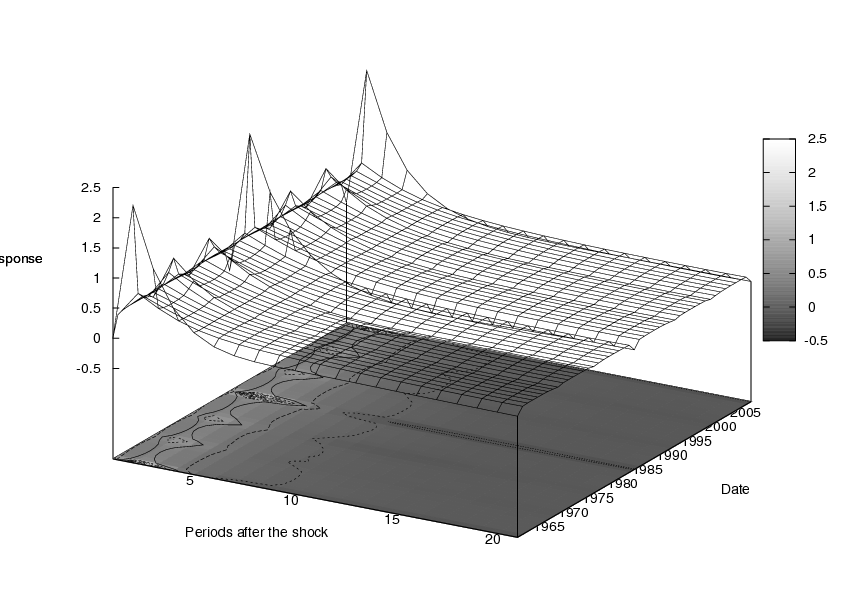
\includegraphics[scale=0.25]{results_reallinit/Inflation_costshock_irf3d.png} \\ \\ 
\multicolumn{2}{c}{Case 3: Learning with Unobservable Shocks and RE Initial Conditions}\\ \\
Output Gap & Inflation \\ 
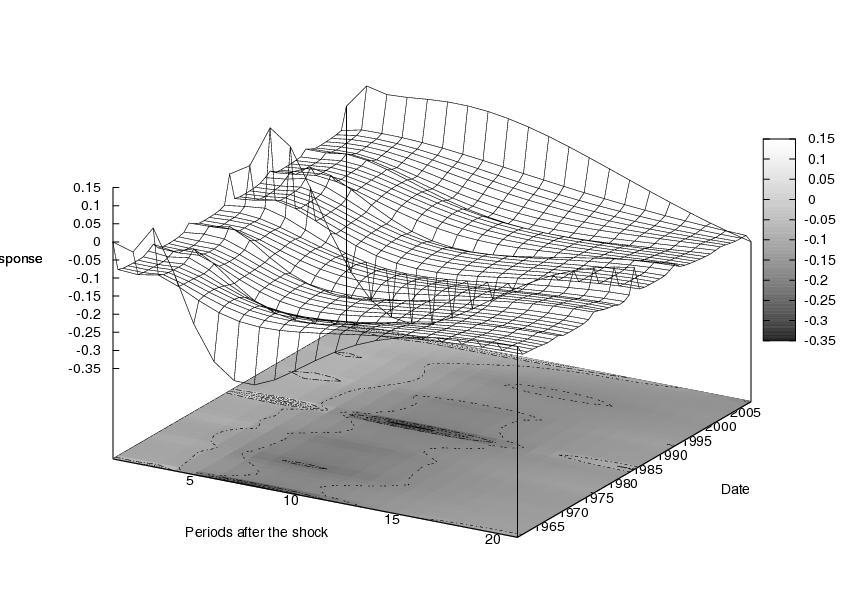
\includegraphics[scale=0.25]{results_reinit/Output_costshock_irf3d.png} & 
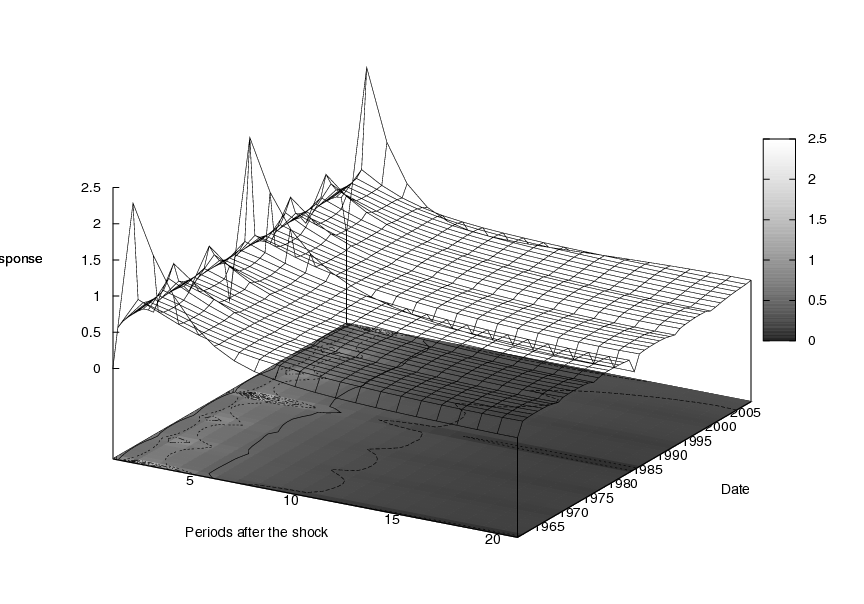
\includegraphics[scale=0.25]{results_reinit/Inflation_costshock_irf3d.png} \\ \\ 
\multicolumn{2}{c}{Case 4: Learning with Unobservable Shocks and Pre-Sample Initial Conditions}\\ \\
Output Gap & Inflation \\ 
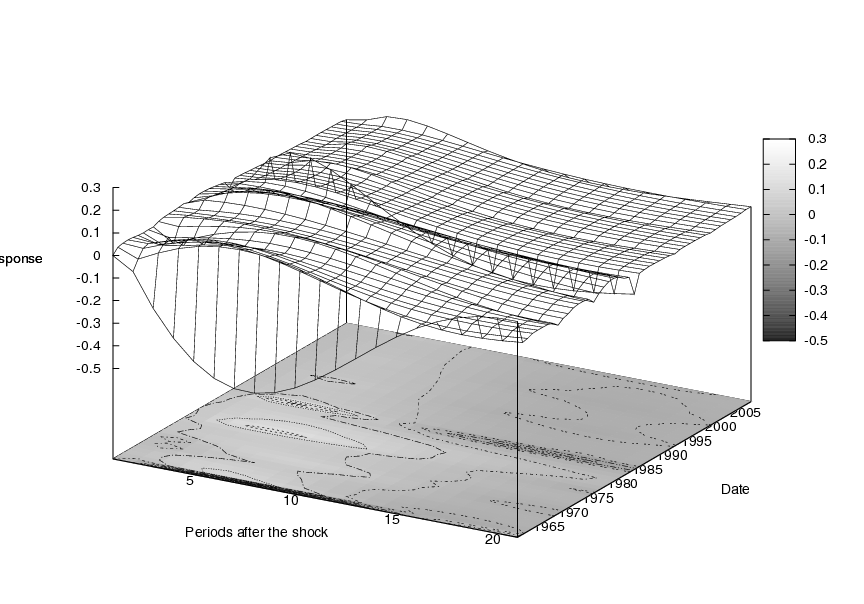
\includegraphics[scale=0.25]{results_wlsinit/Output_costshock_irf3d.png} & 
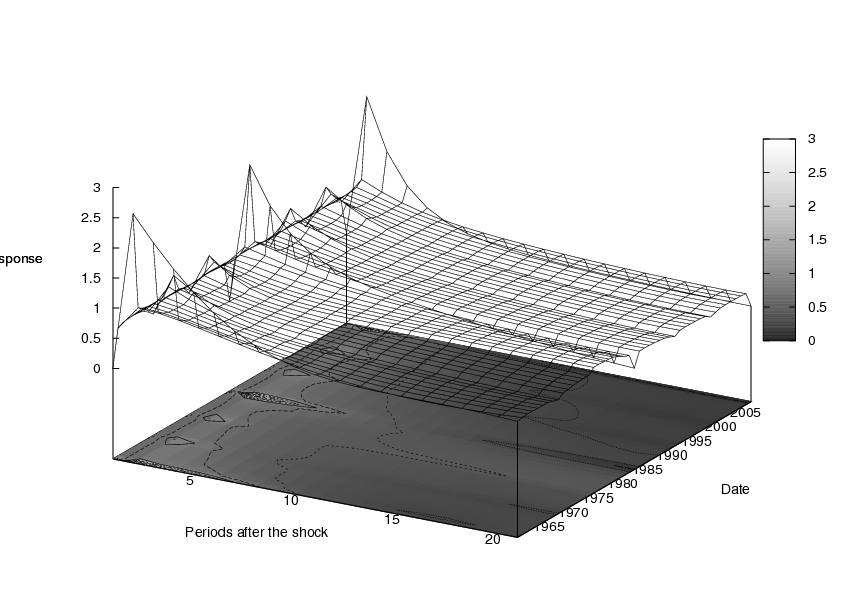
\includegraphics[scale=0.25]{results_wlsinit/Inflation_costshock_irf3d.png} \\ 
\end{tabular}
\end{figure}
